% inspired from http://tex.stackexchange.com/questions/19286/how-should-i-draw-a-singly-double-linked-list
\documentclass{article}

\usepackage{tikz}
\usetikzlibrary{calc, shapes.multipart, chains, arrows}

\begin{document}

% liste chaînée : exemple

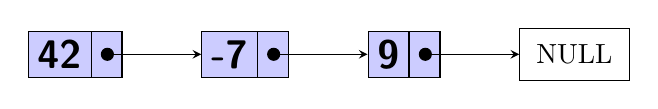
\begin{tikzpicture}[list/.style = {fill = blue!20, font = \sffamily\Large\bfseries, rectangle split, rectangle split parts = 2, draw, rectangle split horizontal}, >=stealth, start chain]
   \node[list, on chain] (A) {42};
   \node[list, on chain] (B) {-7};
   \node[list, on chain] (C) {9};
   \node[on chain, draw, inner sep = 6pt] (D) {NULL};
   \draw[*->] let \p1 = (A.two), \p2 = (A.center) in (\x1,\y2) -- (B);
   \draw[*->] let \p1 = (B.two), \p2 = (B.center) in (\x1,\y2) -- (C);
   \draw[*->] let \p1 = (C.two), \p2 = (C.center) in (\x1,\y2) -- (D);
\end{tikzpicture}

% liste chaînée : exemple ajout élément

\vspace{3cm}
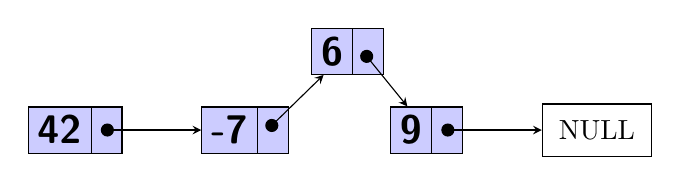
\begin{tikzpicture}[list/.style = {fill = blue!20, font = \sffamily\Large\bfseries, rectangle split, rectangle split parts = 2, draw, rectangle split horizontal}, >=stealth, start chain]
   \node[list, on chain] (A) {42};
   \node[list, on chain] (B) {-7};
   \node[list, on chain] (E) at (2, 1) {6};
   \node[list, on chain] (C) at (3, 0) {9};
   \node[on chain, draw, inner sep = 6pt] (D) {NULL};
   \draw[*->] let \p1 = (A.two), \p2 = (A.center) in (\x1,\y2) -- (B);
   \draw[*->] let \p1 = (B.two), \p2 = (B.center) in (\x1,\y2) -- (E);
   \draw[*->] let \p1 = (E.two), \p2 = (E.center) in (\x1,\y2) -- (C);
   \draw[*->] let \p1 = (C.two), \p2 = (C.center) in (\x1,\y2) -- (D);
\end{tikzpicture}

% liste chaînée : exemple suppression élément

\vspace{3cm}
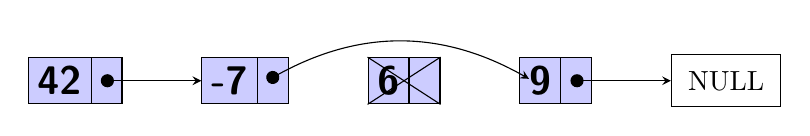
\begin{tikzpicture}[list/.style = {fill = blue!20, font = \sffamily\Large\bfseries, rectangle split, rectangle split parts = 2, draw, rectangle split horizontal}, >=stealth, start chain]
   \node[list, on chain] (A) {42};
   \node[list, on chain] (B) {-7};
   \node[list, on chain] (E) {6};
   \node[list, on chain] (C) {9};
   \node[on chain, draw, inner sep = 6pt] (D) {NULL};
   \draw (E.north east) -- (E.south west);
   \draw (E.north west) -- (E.south east);
   \draw[*->] let \p1 = (A.two), \p2 = (A.center) in (\x1,\y2) -- (B);
   \path[*->] let \p1 = (B.two), \p2 = (B.center) in (\x1,\y2) edge [bend left] ($(C.one) + (0,0.2)$);
   \draw[*->] let \p1 = (C.two), \p2 = (C.center) in (\x1,\y2) -- (D);
\end{tikzpicture}

% liste doublement chaînée : exemple

\vspace{3cm}

\begin{tikzpicture}[list/.style = {fill = blue!20, font = \sffamily\Large\bfseries, rectangle split, rectangle split parts = 3, draw, rectangle split horizontal}, >=stealth, start chain]
   \node[list, on chain] (A) {\nodepart{second}42};
   \node[list, on chain] (B) {\nodepart{second}-7};
   \node[list, on chain] (C) {\nodepart{second}9};
   \node[on chain, draw, inner sep = 6pt] (D) [right = of C] {NULL};
   \node[on chain, draw, inner sep = 6pt] (E) [left =  of A] {NULL};
   \path[*->] let \p1 = (A.three), \p2 = (A.center) in (\x1,\y2) edge [bend left] ($(B.one) + (0,0.2)$);
   \path[*->] let \p1 = (B.three), \p2 = (B.center) in (\x1,\y2) edge [bend left] ($(C.one) + (0,0.2)$);
   \draw[*->] let \p1 = (C.three), \p2 = (C.center) in (\x1,\y2) -- (D);
   \draw[*->] ($(A.one) + (0.2,0.1)$) -- (E);
   \path[*->] ($(B.one) + (0.1,0.1)$) edge [bend left] ($(A.three) + (0,-0.05)$);
   \path[*->] ($(C.one) + (0.1,0.1)$) edge [bend left] ($(B.three) + (0,-0.05)$);
\end{tikzpicture}

% liste chaînée circulaire : exemple

\vspace{3cm}
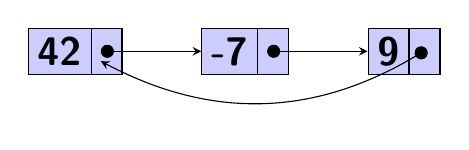
\begin{tikzpicture}[list/.style = {fill = blue!20, font = \sffamily\Large\bfseries, rectangle split, rectangle split parts = 2, draw, rectangle split horizontal}, >=stealth, start chain]
   \node[list, on chain] (A) {42};
   \node[list, on chain] (B) {-7};
   \node[list, on chain] (C) {9};
   \draw[*->] let \p1 = (A.two), \p2 = (A.center) in (\x1,\y2) -- (B);
   \draw[*->] let \p1 = (B.two), \p2 = (B.center) in (\x1,\y2) -- (C);
   \path[*->] ($(C.second) + (0.1,0.1)$) edge [bend left] ($(A.two) + (0,-0.05)$);
\end{tikzpicture}

% liste doublement chaînée circulaire : exemple

\vspace{3cm}
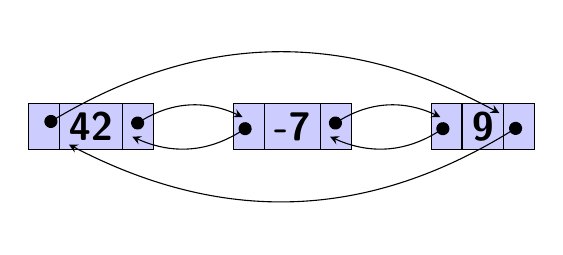
\begin{tikzpicture}[list/.style = {fill = blue!20, font = \sffamily\Large\bfseries, rectangle split, rectangle split parts = 3, draw, rectangle split horizontal}, >=stealth, start chain]
   \node[list, on chain] (A) {\nodepart{second}42};
   \node[list, on chain] (B) {\nodepart{second}-7};
   \node[list, on chain] (C) {\nodepart{second}9};
   \path[*->] let \p1 = (A.three), \p2 = (A.center) in (\x1,\y2) edge [bend left] ($(B.one) + (0,0.2)$);
   \path[*->] let \p1 = (B.three), \p2 = (B.center) in (\x1,\y2) edge [bend left] ($(C.one) + (0,0.2)$);
   \path[*->] ($(B.one) + (0.1,0.1)$) edge [bend left] ($(A.three) + (0,-0.05)$);
   \path[*->] ($(C.one) + (0.1,0.1)$) edge [bend left] ($(B.three) + (0,-0.05)$);
   \path[*->] ($(C.three) + (0.1,0.1)$) edge [bend left] ($(A.two) + (0,-0.05)$);
   \path[*->] ($(A.one) + (0.1,0.1)$) edge [bend left] ($(C.two) + (0.35,0.35)$);
\end{tikzpicture}

\end{document}
